First we consider about the $2*2$ mesh network,  which can be generalized to a $2*n$ mesh network.  After, we analyze a more general case $m*n$ mesh network and obtain a general closed-form matrix presentation.  Finally, we give a key methodology to address this type of question.  In addition, different single data injection position, such as the corner, boundary and inner grid are also discussed.  

The load $L$ is assigned on the corner processor $P_{0}$ Fig ~\ref{fig:2t2}.  The whole task is tackled by four processors $P_{0}$, $P_{1}$, $P_{2}$, $P_{3}$ together.  

\begin{figure}[!ht]
\centering
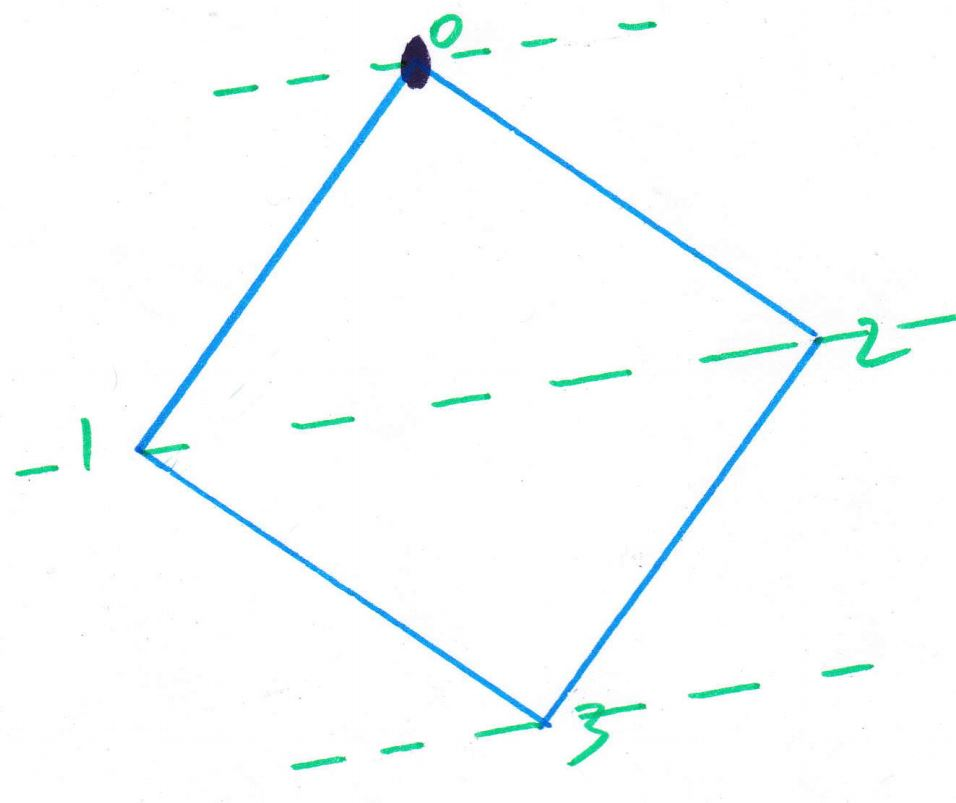
\includegraphics[width=0.5\columnwidth]{figure/2t2.JPG}
\caption{The 2*2 mesh network and the root processor is $P_{0}$}
\label{fig:2t2}
\end{figure}

The processor $P_{0}$, $P_{1}$ and $P_{2}$ start to process its respective fraction at the same time.  This includes $P_{1}$ and $P_{2}$ as they are relayed load in virtual cut-through mode at $t = 0$.  The processor $P_{3}$ starts to work when the $\alpha_{1}$ and $\alpha_{2}$ complete transmission.  That is, the link $0-1$ and $0-2$ are occupied 
transmitting load to processor $1$ and $2$, respectively and only transmission to $3$ when that is finished.
According to the divisible load theory  \cite{bharadwaj2003divisible}, we obtain the timing diagram Fig ~\ref{fig:2t2d}.  

\begin{figure}[!ht]
\centering
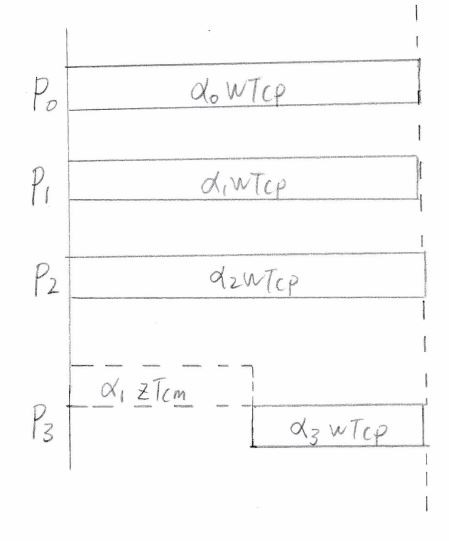
\includegraphics[width=0.5\columnwidth]{figure/2t2d.JPG}
\caption{The timing diagram for 2*2 mesh network and the root processor is $P_{0}$}
\label{fig:2t2d}
\end{figure}

Here in the Gantt-like timing diagram communication appears above each axis and computations appears below the each axis.  Let's assume that all processors stop computing at the same time in order to minimize the makespan  \cite{sohn1992optimal}.

Based on the timing diagram, we obtain a group of linear equations to find the fraction workload assigned to each processor $\alpha_{i}$ : 

\begin{empheq}[left=\empheqlbrace]
{align}
\alpha_{0} \omega T_{cp} = T_{f, m}\\
\alpha_{1} \omega T_{cp} = T_{f, m}\\
\alpha_{2} \omega T_{cp} = T_{f, m}\\
\alpha_{1}zT_{cm} + \alpha_{3}\omega T_{cp} = T_{f, m}\\
\alpha_{0} + \alpha_{1} + \alpha_{2} + \alpha_{3} = 1\\
\sigma = \frac{zT_{cm}}{\omega T_{cp}}\\
0 < \sigma < 1 \\
0 < \alpha_{0} \leq  1\\
0 \leq  \alpha_{1},  \alpha_{2},  \alpha_{3}  < 1
\end{empheq}
\\

The group of equations are represented by the matrix form:

\begin{equation}
{
\left[ \begin{array}{ccc}
1 & 2 & 1\\
1 & -1 & 0\\
0 & \sigma-1 & 1
\end{array} 
\right ]} \times \left[ \begin{array}{c}
\alpha_{0} \\
\alpha_{1} \\
\alpha_{3} 
\end{array} 
\right ] = \left[ \begin{array}{c}
1 \\
0 \\
0 
\end{array} 
\right ]
\end{equation}
The matrix is represented as $A \times \alpha = b$.  $A$ is named as the \textbf{\textit{flow matrix}}.
Here because of symmetry $\alpha_{1} = \alpha_{2}$, so $\alpha_{2}$ is not listed in the matrix equations.

Finally, the explicit solution is:
\begin{empheq}[left=\empheqlbrace]
{align}
\sigma = \frac{zT_{cm}}{\omega T_{cp}}\\
\alpha_{0} = \frac{1}{4- \sigma}\\
\alpha_{1} = \frac{1}{4- \sigma}\\
\alpha_{3} = \frac{1 - \sigma}{4- \sigma}
\end{empheq}
\\
The equations say that as $\sigma$ grows,  the value $\alpha_{3}$ drops.  In other words, as the communication capacity decreases, there is less data workload assigned to $P_{3}$.  Further, it means it will be economical to keep the load local on $P_{0}$ $P_{1}$ $P_{2}$ and not distribute it, to other processors.  

The equivalence inverse speed of a a single processor is $w_{eq}$, that can replace the original network as
$$T_{f,n} = 1*w_{eq}*T_{cp}$$
$$w_{eq} = \alpha_{0}*w$$
$$Speedup = \frac{T_{f, 0}}{T_{f, n}}= \frac{\omega T_{cp}}{\alpha_{0}\omega T_{cp}} = \frac{1}{\alpha_{0}} = 4- \sigma$$